\documentclass[a4paper,11pt,DIV=16,parskip=half,ngerman]{scrartcl}
\usepackage{graphicx}
\graphicspath{{../../Code/211/Diagramme}}
\usepackage{pdfpages}

\usepackage[utf8]{inputenc}                     % for using utf8 chars (äöüß)
\usepackage[T1]{fontenc}                        % for correct font encoding (you 
                                                % can't search for non-ascii 
                                                % chars in pdf otherwise)
\usepackage{lmodern}
\usepackage{microtype}
\usepackage[ngerman]{babel}             
% \usepackage{amsmath}
% \usepackage{amssymb}                           
\usepackage{csquotes}
\begin{document}
Die Auswirkung der Reibungseffekte auf die FFT konnte ich mir anhand der mathematischen Formel nicht vorstellen. Deswegen habe ich jetzt die FFT der Funktion \(f_{reib}=e^{-\delta t}\cdot \varphi_0 \cos{\omega_1 t}\) geplottet. \(\delta\) habe ich rudimentär aus zwei Messpunkten der \verb|tx(t)| Datei berechnet. 
\begin{figure}[h!]
    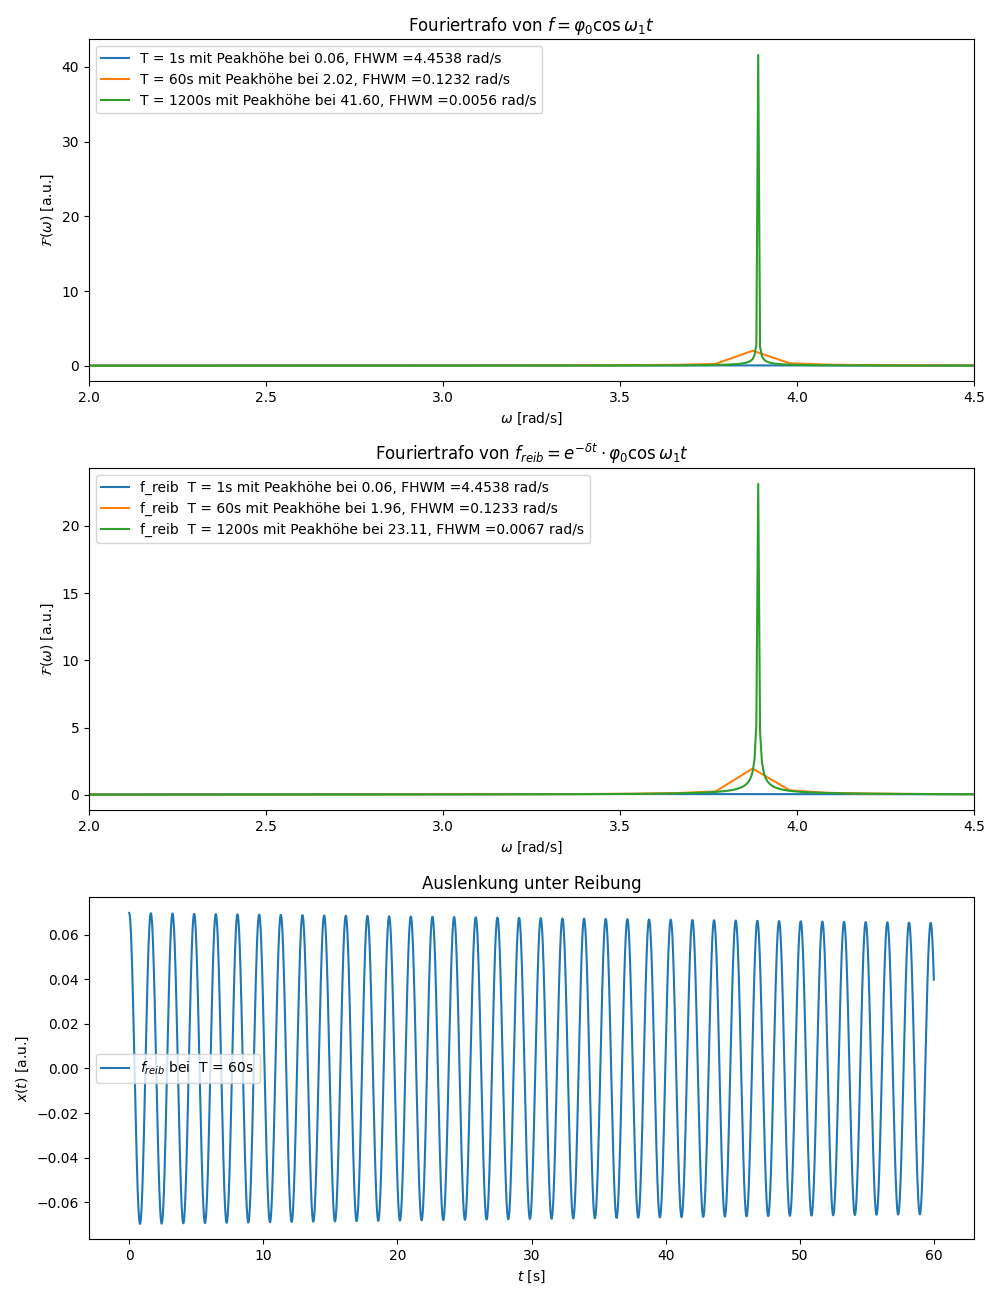
\includegraphics[width=\textwidth]{Fouriertrafos.png}
\end{figure}
\clearpage
Man sieht, die Amplitude der Peaks sinkt, die FHWM wird jedoch nur bei nicht signifikanten Stellen minimal größer. Auch die x-Stelle der Peaks, also die Frequenz \(\omega_1\) bleibt am exakt gleichen Ort. \\
Reibungseffekte können also komplett vernachlässigt werden. \par
Nun die Frage: Warum schreibst du aber in der Diskussionshilfe: \enquote{[mit dem Wissen, dass] Reibung einem/einer einen Strich durch die Rechnung machen wird[...]}. Das impliziert, das Reibung die Messergebnisse signifikant verfälscht hat, was aber nach den Plots nicht so ist. 
\includepdf[pages=9-]{../../Code/211/2111.pdf}

\end{document}
